


\chapter{Conclusions}

In this thesis, after presenting the main theoretical concepts and the main instruments (hardware and software) used, I focused on the characterization and calibration experiments required to fully control a superconducting quantum device.
A detailed description of all the experiments has been provided along with ideal and real plots for different scenarios.

\paragraph{Software development}

Although the explanation of these experiments is the main part of this thesis, the time spent at the Technology Innovation Institute was in large part dedicated to develop the software tools required for the experiments themselves.
This included the development of parts of \Qibolab and of \Qibosoq of which some details were given in \cref{sec:software}.

Both of these software tools are open source and are being officially presented to the research community via papers \cite{Efthymiou_2023} currently under review for the Quantum journal.

It is useful, for the purpose of better explaining my role in the development of these tools, to provide a brief description of them when I first started and when I finished the thesis.\\
When I first arrived, \Qibolab was in an alpha-testing phase and was not fully released yet.
Remember that the main idea behind \Qibolab is to support, with the same interface, multiple devices and instruments.
At that time, however, it supported only Quantum Machines devices and some Qblox devices (with outdated firmware).
My main role was to add to \Qibolab the full support of the RFSoC FPGAs compatible with the \Qick project, but I also worked in the development of the general interface, helping reaching the first stable release of the software.

For what concerns \Qibosoq, when I first arrived at TII, it was nothing but a prototype script, it was not compatible with the \Qibolab interface and therefore was not of any real use.
I developed it to the first stable release and reached a stage were all the major features supported by \Qick and \Qibolab are supported and integrated in the software.\\
The role of \Qibosoq could be critical for the research community, since it creates a connection between an open source software for control, \Qibolab, and a high-precision and economically-feasible hardware solution as the RFSoCs and \Qick.

\paragraph{Calibration experiments}

To develop and test the software solutions introduced in \Qibolab and \Qibosoq, continuous hardware testing on real qubits was required, as well as the software implementation of various calibration and characterization experiments.

In this thesis, I detailed the experiments required to fully calibrate a single qubit device, as well as the first main experiments required for two-qubit gates calibration. 
I tried to set up the calibration sections as a practical manual, so that it may be used by novice experimenters in the future.
Indeed many more experiments can be developed to increase readout and gate fidelities, but following the layout of routines detailed in this thesis will give full and acceptable control capacities on a standard superconducting qubit.
Moreover, the user of this ''manual`` will also gain a good enough knowledge on the underlying quantum-mechanical and cQED principles exploited for readout and control.
A small list of other possible calibration experiments was also provided in \cref{sec:other_possible}, to show the ''infinite`` possible number of experiments.

\paragraph{Algorithmic applications}

The RFSoC-based setup I developed during this thesis, along with the qubits I characterized and calibrated, was already used both by me and by other colleagues with no knowledge of the underlying complexity of \Qibosoq and \Qick. 
This demonstrates how relevant it is to produce a tool with a simple interface, that can be used by experimenters without needing to split focus between software and the experiment itself.

\Qibosoq has been used for algorithmic applications, of which the fitting procedure in \cref{sec:qml_application} is an example.
Moreover, it has also been used to develop a generative quantum neural network (article soon to be published).

In general, the RFSoC-based system has been proved to be as reliable as the commercial solutions and slightly faster than those, in particular for circuit-based experiments (so algorithmic applications) as presented in \cref{fig:benchmark}~\cite{qibosoq_paper, Efthymiou_2023}.

\begin{figure}[ht]
    \centering
    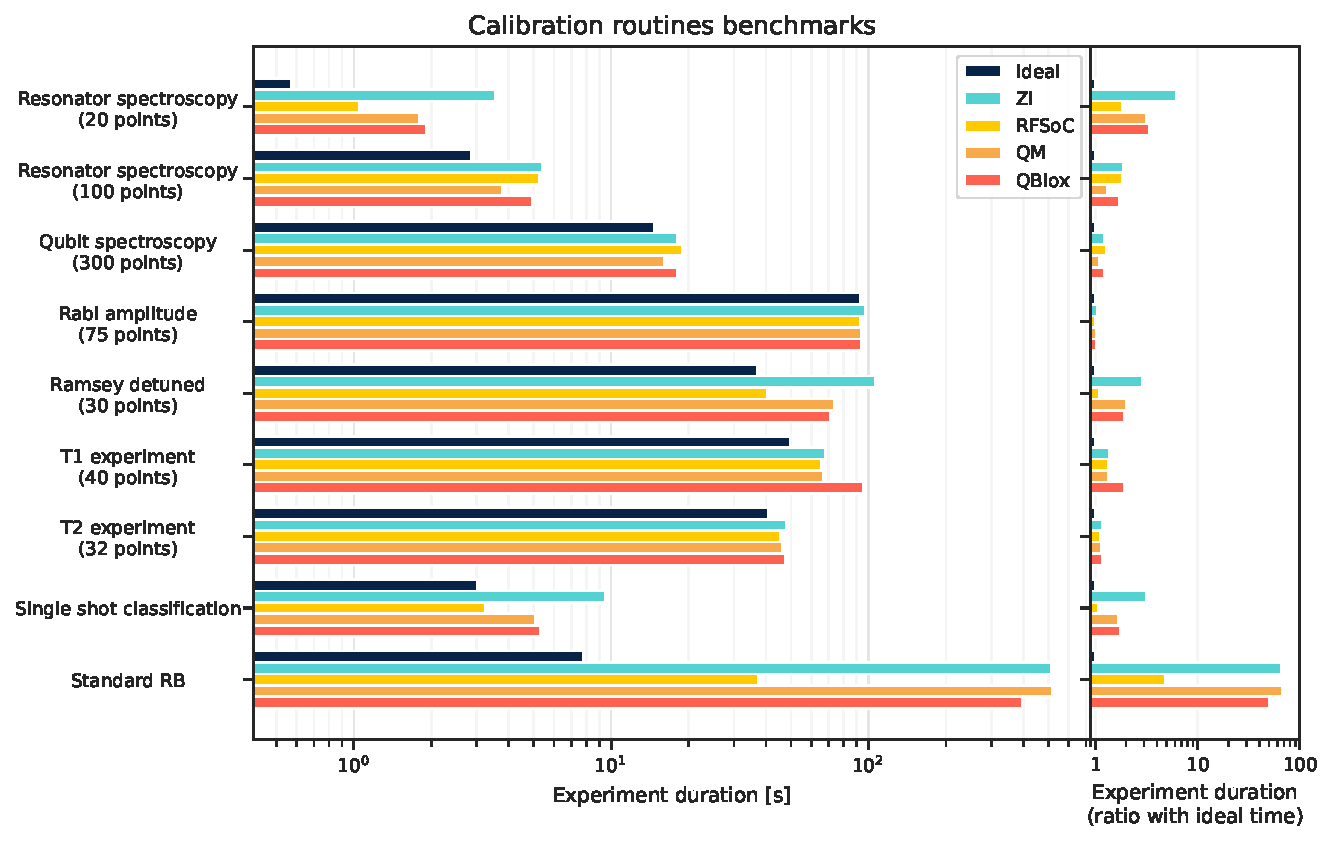
\includegraphics[width=\textwidth]{Other sections/figures/routines.pdf}
    \caption[Speed benchmark of a \Qibosoq system Vs. commercial alternatives]{Execution time of different qubit calibration routines on various electronics. On the left side there is the absolute times in seconds for each experiment. The ideal time (black bar) shows the minimum time the qubit needs to be affected in each experiment. On the right side the ratio between actual execution time and ideal time is shown.}
    \label{fig:benchmark}
\end{figure}


\paragraph{Outlook and quantum sensing applications}

For the moment, \Qibosoq and the RFSoC-based setup was used just for computing applications.
The software too was developed with only calibration experiments and circuits applications in mind.

To fully unlock the potential of qubits in the particle physics research world, however, and in particular to offer \Qibosoq as a complete control solution, independently from the type of final use, some development and testing is still needed.

Various experimental protocols are already been proposed to use qubits as detectors and, in any case, quantum sensing is one of the most interesting active topic of research in quantum technologies.
The experiment presented in \cref{sec:sens_application} is an example of feasible application.

Note that the majority of elements required for sensing (in general, we are always talking about pulses and measurements) are already supported, but some changes in the interface and some more features are required to make \Qibosoq a reliable tool (for example, the support for continuous acquisition modes).

Moreover, RFSoC FPGAs are not limited to the control of superconducting qubits and could be used also for different types of technologies such as photonic quantum computing (with also some hardware modification).

In the future, \Qibosoq will be extended for applications different from quantum computing and, in particular, for quantum sensing researches.